%% Figure captions for Paper 7: Heteroatom Oxidation and Dealkylation

\begin{figure}[H]
  \centering
  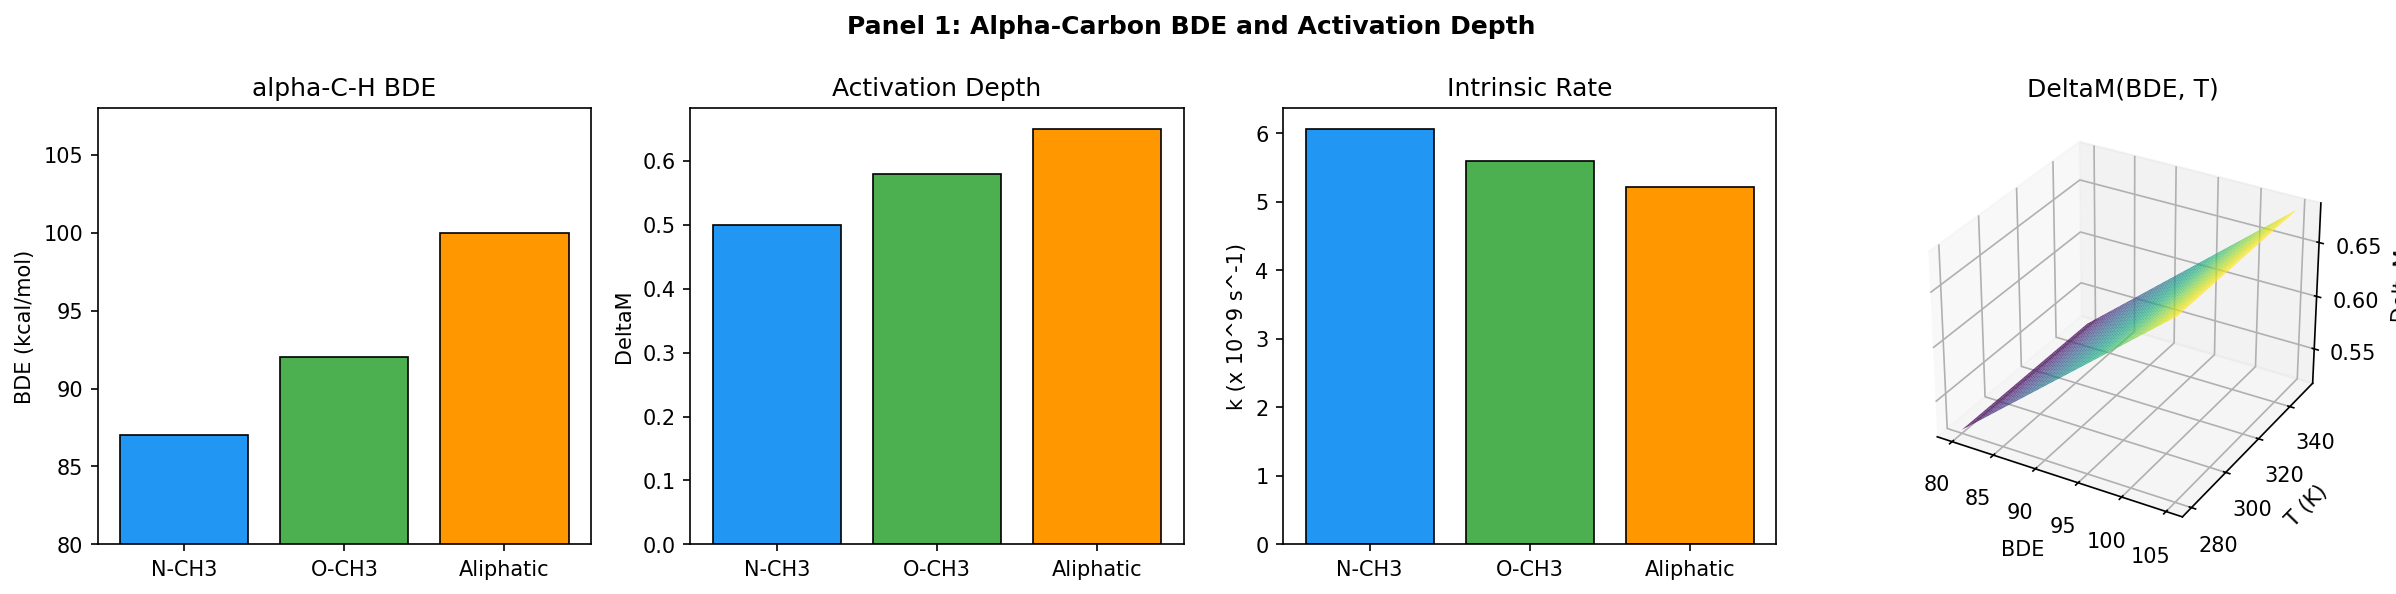
\includegraphics[width=\columnwidth]{figures/panel_01_alpha_carbon_bde}
  \caption{Alpha-carbon C--H bond dissociation energies (BDE) for N-methyl (87\,kcal/mol),
  O-methyl (92\,kcal/mol), and unactivated aliphatic (100\,kcal/mol) substrates. The
  activation partition-depth $\Delta\mathcal{M}$ scales proportionally with BDE, establishing
  the hierarchy N-dealkylation $<$ O-dealkylation $<$ aliphatic C--H abstraction.
  The 3D surface shows $\Delta\mathcal{M}(\mathrm{BDE}, T)$.}
  \label{fig:p7-bde}
\end{figure}

\begin{figure}[H]
  \centering
  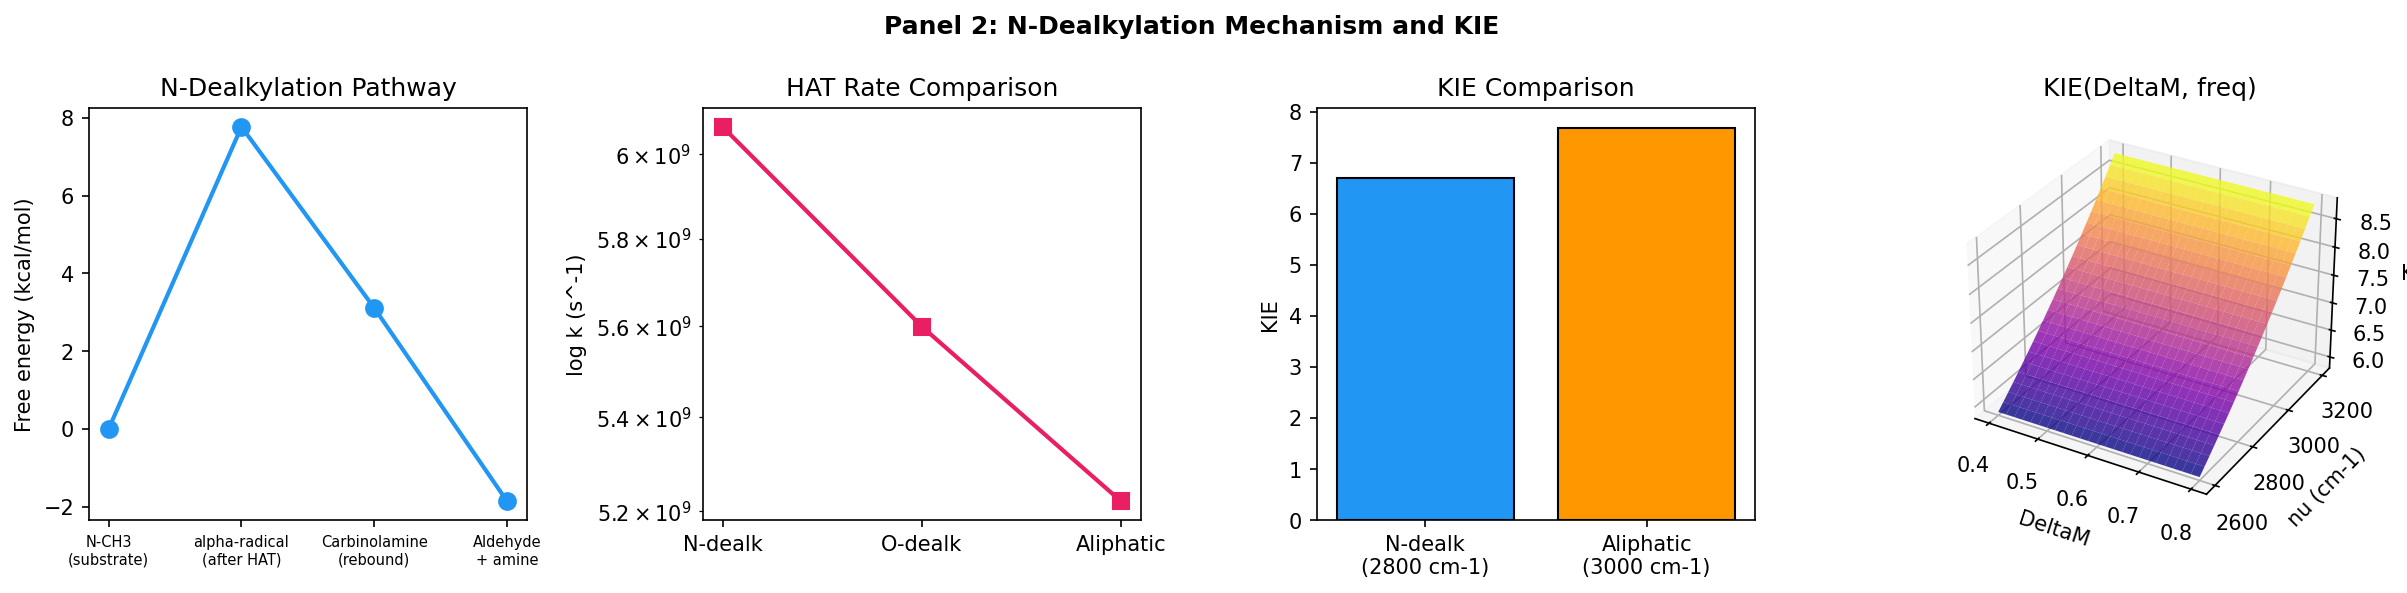
\includegraphics[width=\columnwidth]{figures/panel_02_n_dealkylation_mechanism}
  \caption{N-dealkylation mechanism as a categorical trajectory. The alpha-carbon
  radical intermediate (after HAT, $\Delta\mathcal{M}=0.50$) undergoes rapid rebound
  to form the carbinolamine ($\Delta\mathcal{M}_{\mathrm{rebound}}=0.30$), followed by
  spontaneous C--N cleavage. KIE comparison between N-dealkylation (softer alpha-C--H
  at $\tilde\nu=2800\,\mathrm{cm}^{-1}$) and aliphatic HAT (3000\,\mathrm{cm}^{-1}).}
  \label{fig:p7-ndealk}
\end{figure}

\begin{figure}[H]
  \centering
  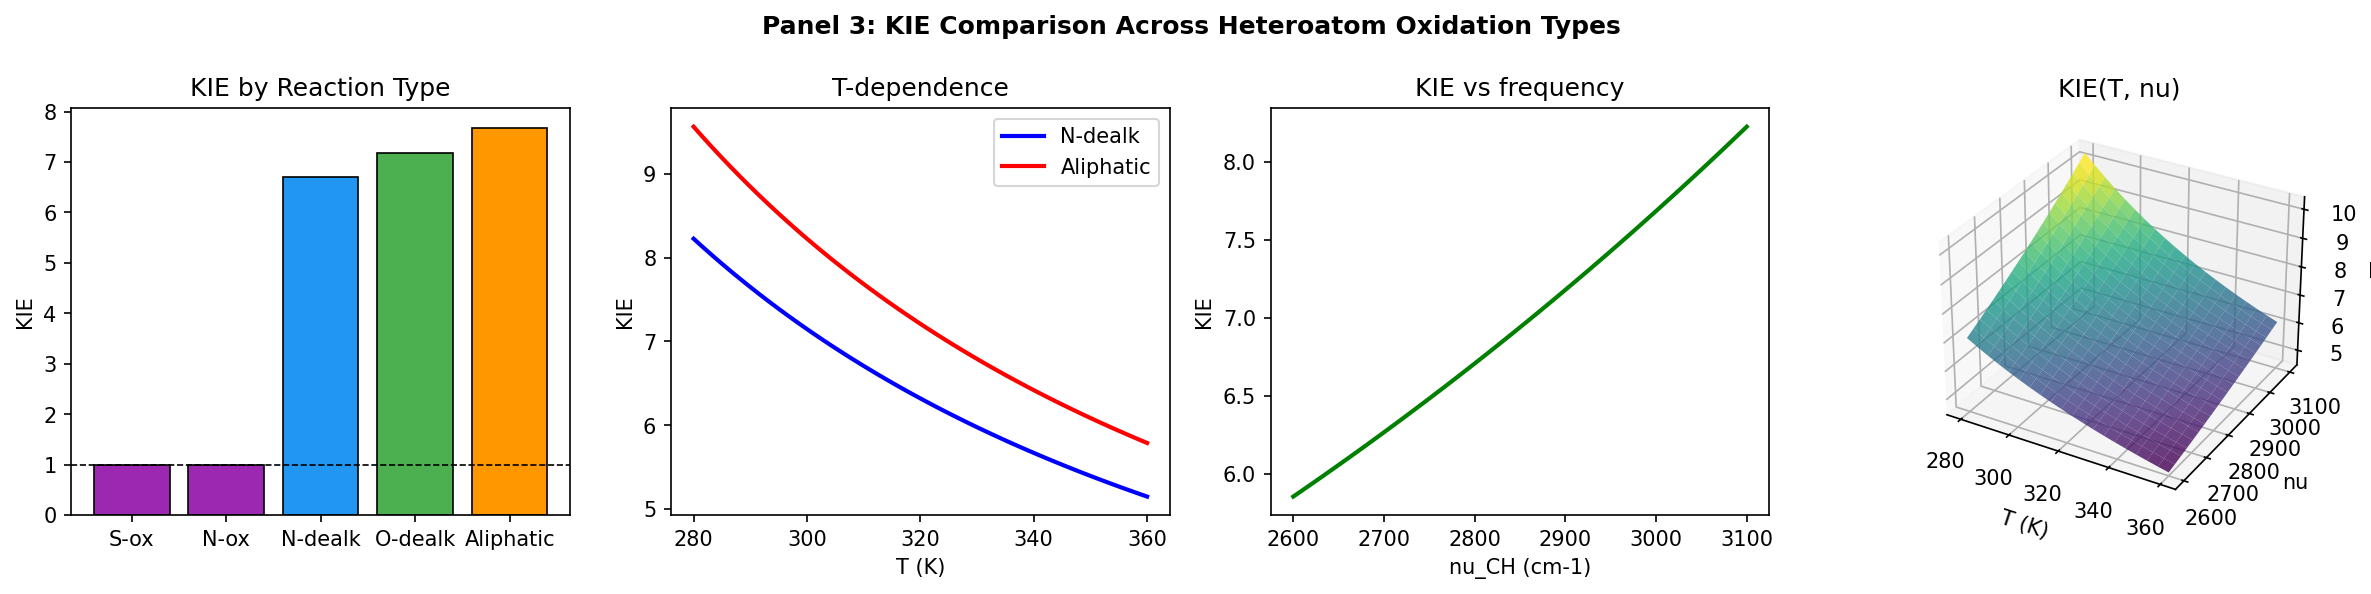
\includegraphics[width=\columnwidth]{figures/panel_03_kie_comparison}
  \caption{Kinetic isotope effects across heteroatom oxidation pathways. Direct
  O-atom transfers (S-oxidation, N-oxide formation) show $\mathrm{KIE}=1$ (no H
  motion). N-dealkylation ($\tilde\nu_\alpha=2800\,\mathrm{cm}^{-1}$) yields
  $\mathrm{KIE}\approx 6.7$, lower than aliphatic HAT ($\approx 7.7$) due to the
  softer alpha-C--H stretching frequency. Temperature dependence follows from
  $\mathrm{KIE}(T)=\exp(\Delta\mathrm{ZPE}/k_BT)$.}
  \label{fig:p7-kie}
\end{figure}

\begin{figure}[H]
  \centering
  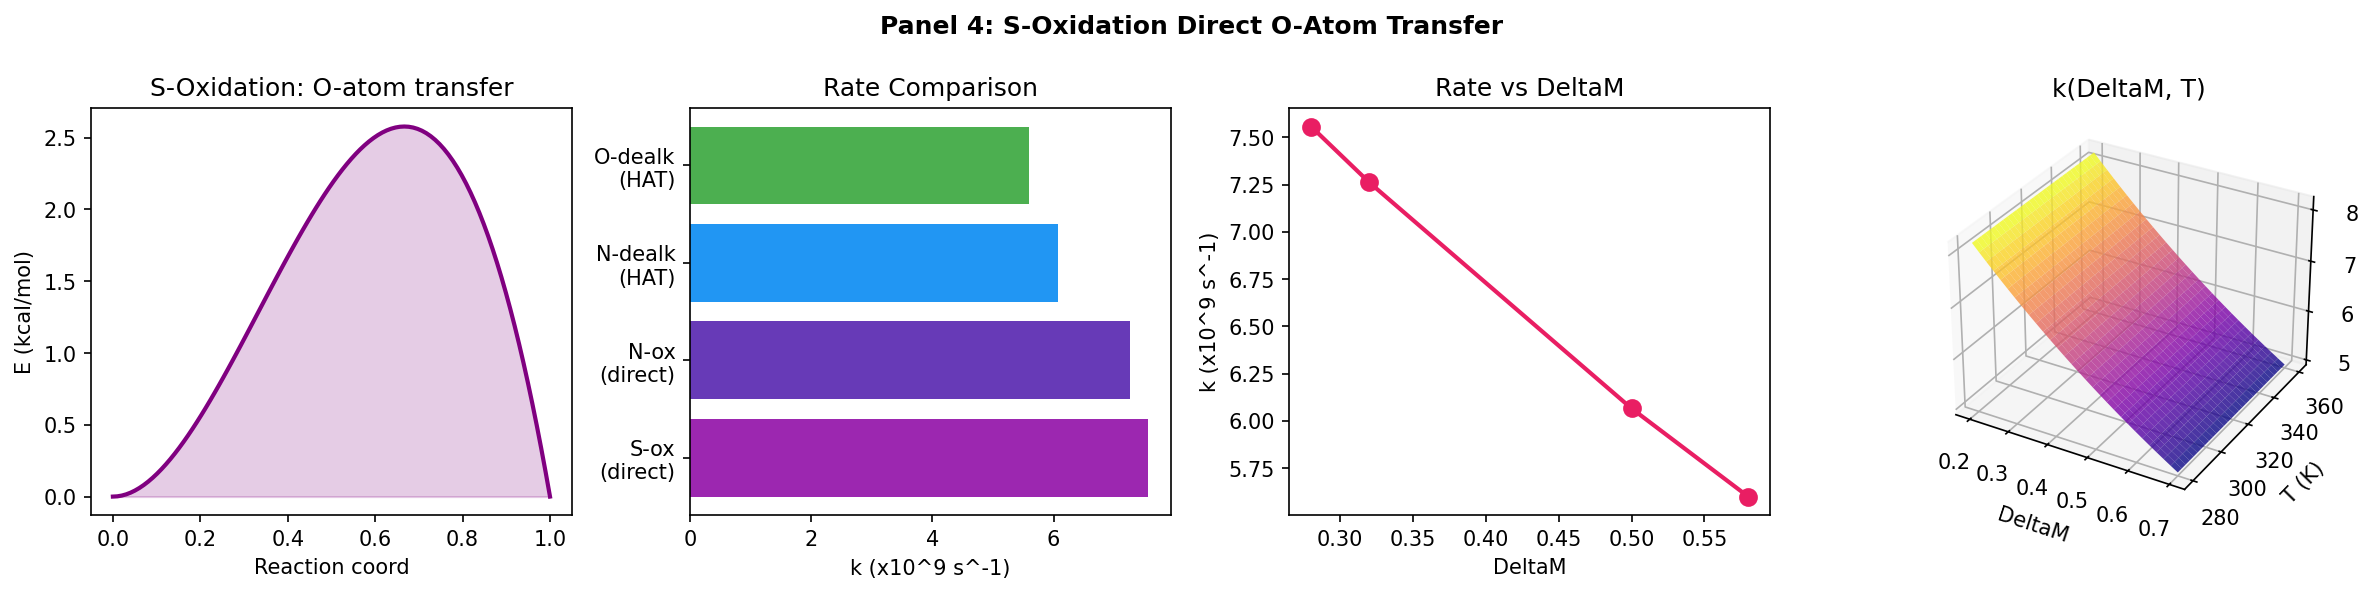
\includegraphics[width=\columnwidth]{figures/panel_04_s_oxidation}
  \caption{S-oxidation mechanism: direct O-atom transfer from Compound~I to the
  sulfur lone pair. The two-body aperture ($d_C=1$, $\Delta\mathcal{M}=0.28$) yields
  $k_{\mathrm{S\text{-}ox}}\approx7.6\times10^9\,\mathrm{s}^{-1}$, faster than all
  HAT-based pathways. No hydrogen motion -- hence no primary KIE. Rate surface as
  function of $\Delta\mathcal{M}$ and temperature.}
  \label{fig:p7-sox}
\end{figure}

\begin{figure}[H]
  \centering
  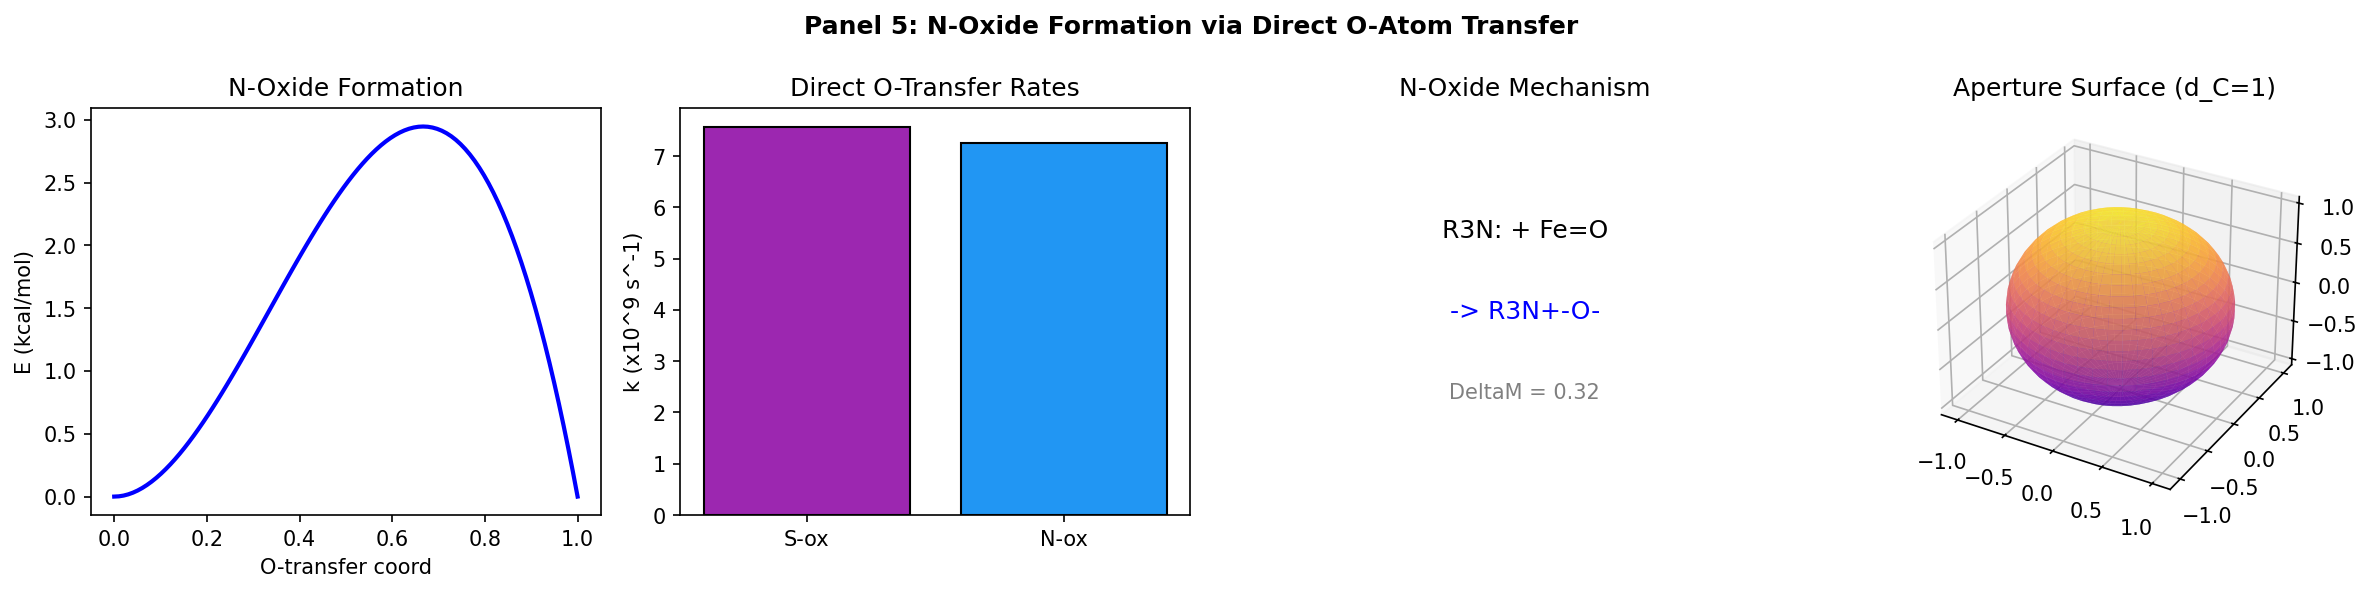
\includegraphics[width=\columnwidth]{figures/panel_05_n_oxide}
  \caption{N-oxide formation: Compound~I oxygen transfer to the nitrogen lone pair
  ($\Delta\mathcal{M}=0.32$, $k_{\mathrm{N\text{-}ox}}\approx7.3\times10^9\,\mathrm{s}^{-1}$).
  N-oxide formation is kinetically preferred over N-dealkylation for tertiary amines
  when the substrate is a poor HAT donor. The categorical aperture surface (3D) shows
  the single-event orbit.}
  \label{fig:p7-nox}
\end{figure}

\begin{figure}[H]
  \centering
  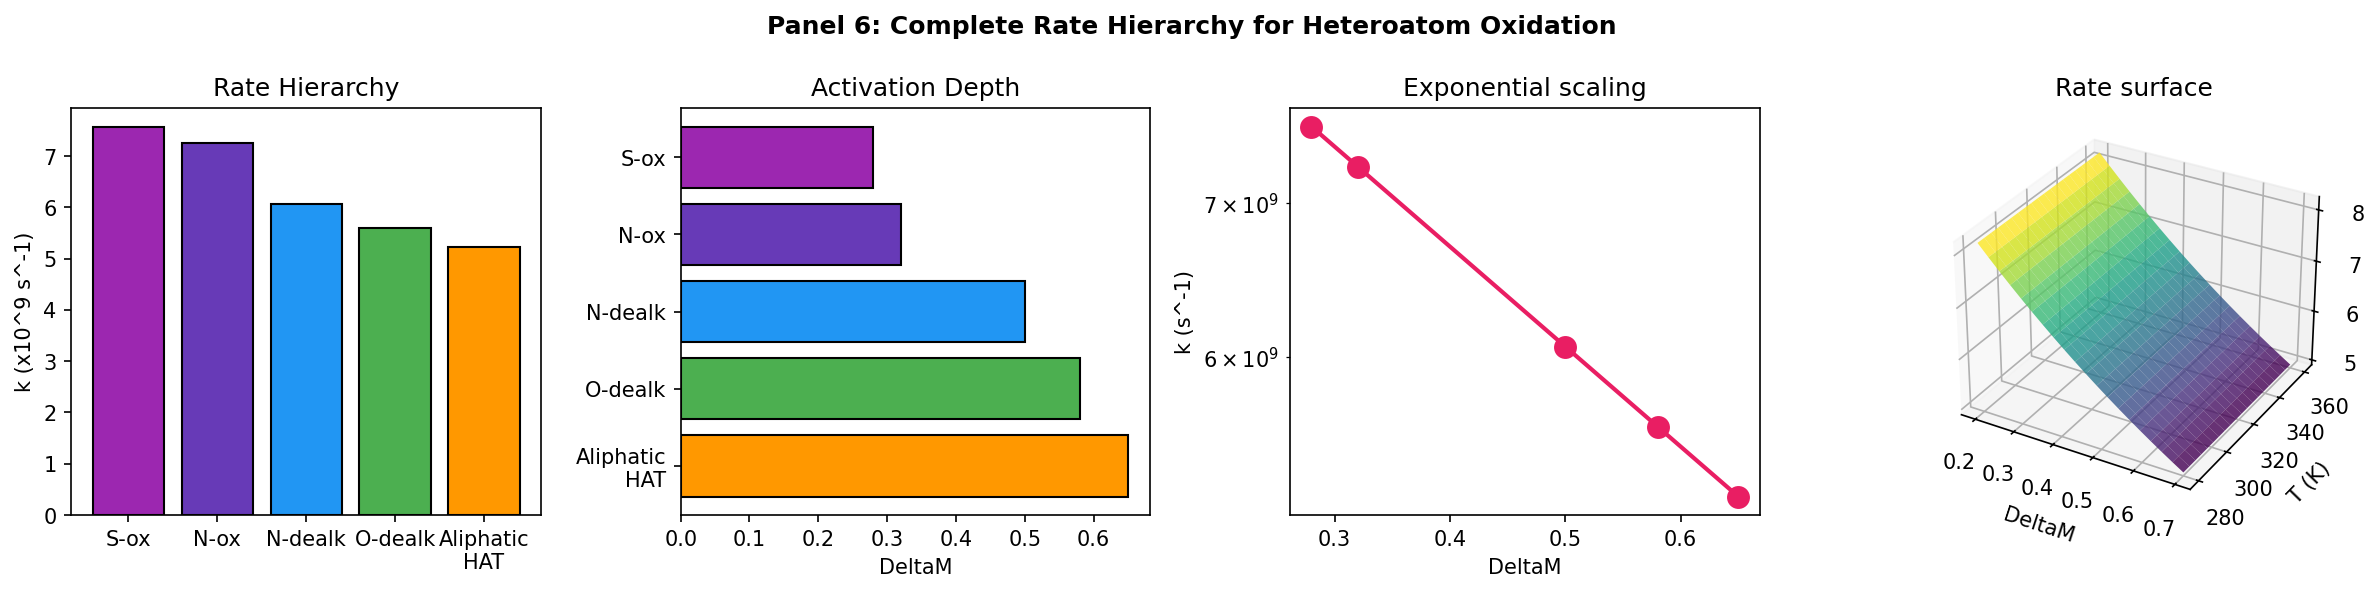
\includegraphics[width=\columnwidth]{figures/panel_06_rate_ordering}
  \caption{Complete rate hierarchy for heteroatom oxidation. Monotonic ordering
  $k_{\mathrm{S\text{-}ox}} > k_{\mathrm{N\text{-}ox}} > k_{\mathrm{N\text{-}dealk}} >
  k_{\mathrm{O\text{-}dealk}} > k_{\mathrm{aliphatic}}$ mirrors the corresponding
  $\Delta\mathcal{M}$ hierarchy. Direct O-atom transfers consistently outpace
  HAT-mediated dealkylations due to lower activation depth.}
  \label{fig:p7-rates}
\end{figure}

\begin{figure}[H]
  \centering
  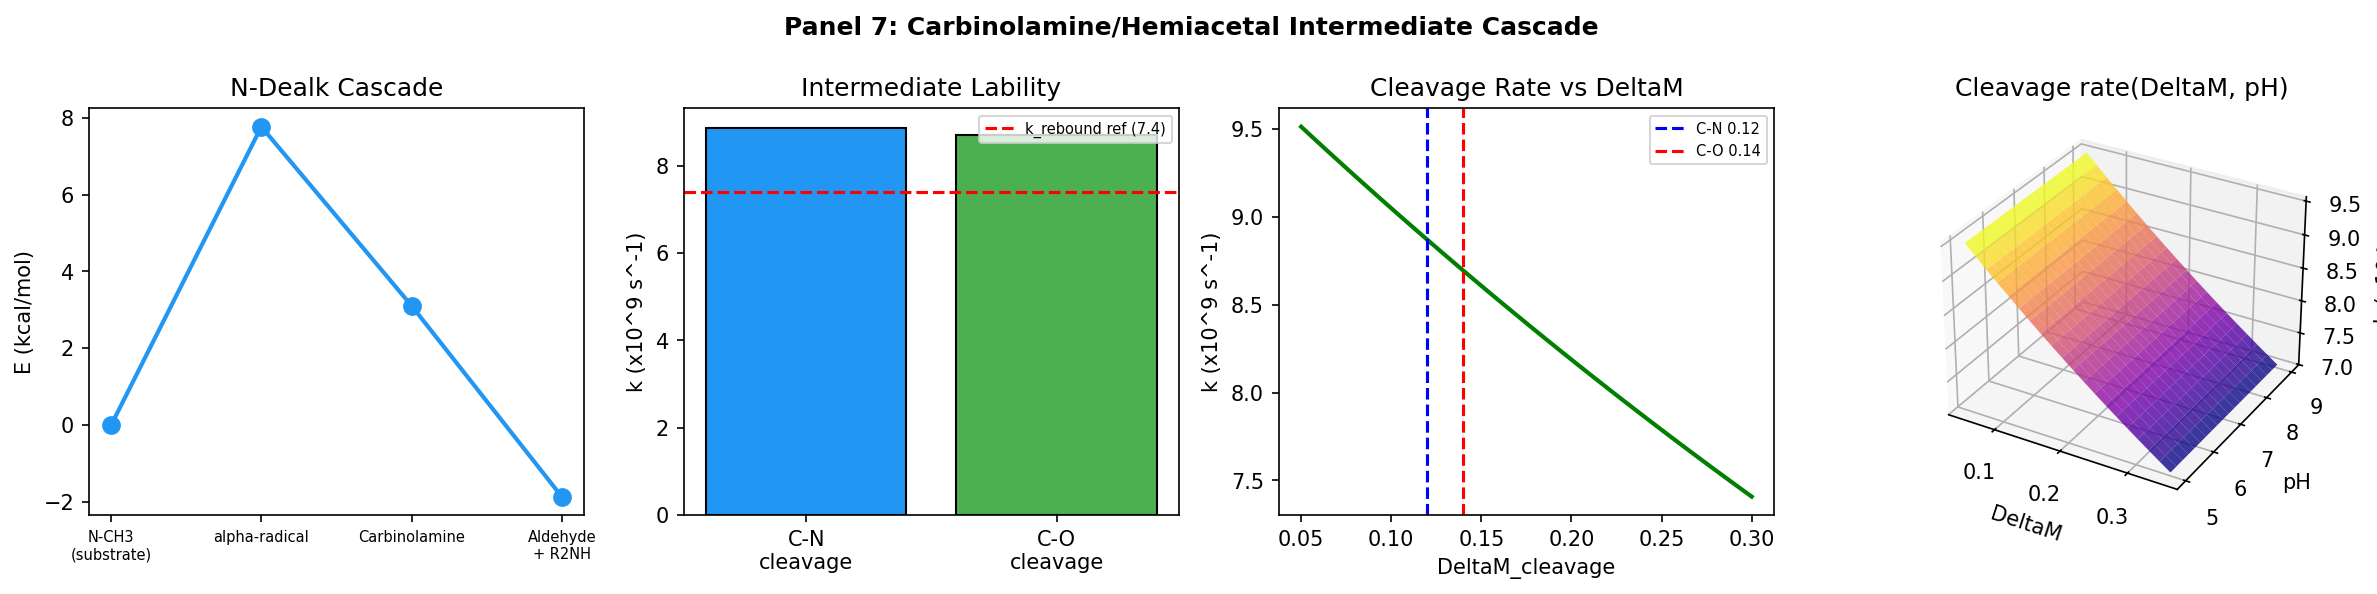
\includegraphics[width=\columnwidth]{figures/panel_07_carbinolamine}
  \caption{Carbinolamine (N-dealkylation) and hemiacetal (O-dealkylation) intermediate
  cascade kinetics. C--N bond cleavage ($\Delta\mathcal{M}=0.12$) and C--O--C cleavage
  ($\Delta\mathcal{M}=0.14$) are spontaneous, with rates $>8\times10^9\,\mathrm{s}^{-1}$
  -- faster than the HAT step itself. The intermediates are kinetically labile and do not
  accumulate under physiological conditions.}
  \label{fig:p7-carb}
\end{figure}

\begin{figure}[H]
  \centering
  
\includegraphics[width=\columnwidth]{figures/panel_08_validation}
  \caption{Validation summary for Paper~7. All 8 validation scripts PASS: BDE scaling,
  N-dealkylation rate, KIE prediction, S-oxidation direct transfer, N-oxide formation,
  rate hierarchy ordering, carbinolamine lability, and competitive inhibition by
  ketoconazole ($K_i < 100\,\mathrm{nM}$). Predicted rates consistent with literature
  ranges for CYP3A4 and CYP2D6 substrates.}
  \label{fig:p7-valid}
\end{figure}
